
\tikzset{every picture/.style={line width=0.75pt}} %set default line width to 0.75pt        
\resizebox{\textwidth}{!}{%
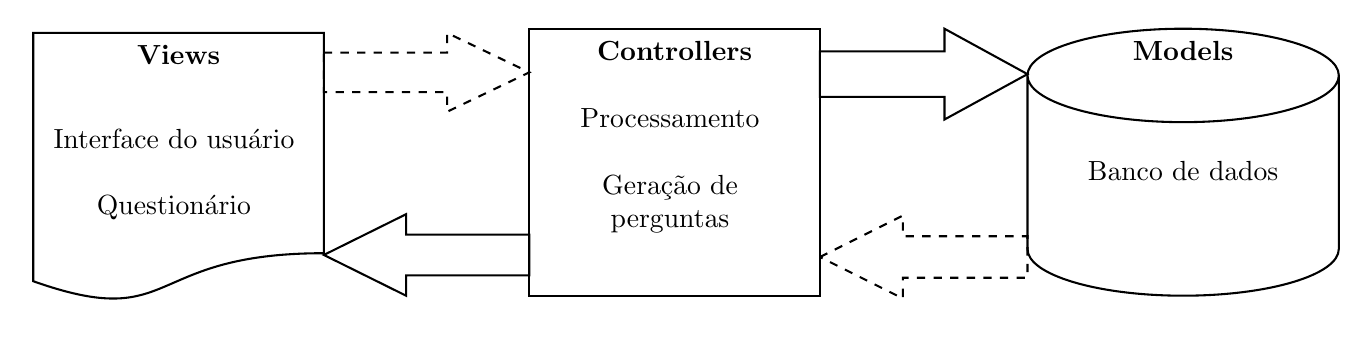
\begin{tikzpicture}[x=0.75pt,y=0.75pt,yscale=-1,xscale=1]
%uncomment if require: \path (0,300); %set diagram left start at 0, and has height of 300

%Flowchart: Magnetic Disk [id:dp16979524550945557] 
\draw (650,102.51) -- (650,186.12) .. controls (650,198.55) and (616.42,208.63) .. (575,208.63) .. controls (533.58,208.63) and (500,198.55) .. (500,186.12) -- (500,102.51)(650,102.51) .. controls (650,114.94) and (616.42,125.02) .. (575,125.02) .. controls (533.58,125.02) and (500,114.94) .. (500,102.51) .. controls (500,90.08) and (533.58,80) .. (575,80) .. controls (616.42,80) and (650,90.08) .. (650,102.51) -- cycle ;
%Flowchart: Document [id:dp9586000142466773] 
\draw (21,82.04) -- (161,82.04) -- (161,188.16) .. controls (73.5,188.16) and (91,226.42) .. (21,201.66) -- cycle ;
%Flowchart: Process [id:dp6310623690046997] 
\draw (260,80) -- (400,80) -- (400,208.63) -- (260,208.63) -- cycle ;
%Right Arrow [id:dp033275286474635735] 
\draw [dashed] (161,91.53) -- (220.4,91.53) -- (220.4,82.04) -- (260,101.02) -- (220.4,120) -- (220.4,110.51) -- (161,110.51) -- cycle ;
%Right Arrow [id:dp9102894989767911] 
\draw (400,90.94) -- (460,90.94) -- (460,80) -- (500,101.88) -- (460,123.76) -- (460,112.82) -- (400,112.82) -- cycle ;
%Left Arrow [id:dp6006547487955811] 
\draw (161,189) -- (200.6,169.38) -- (200.6,179.19) -- (260,179.19) -- (260,198.81) -- (200.6,198.81) -- (200.6,208.63) -- cycle ;
%Left Arrow [id:dp43669281204893773] 
\draw [dashed] (400,190) -- (440,170) -- (440,180) -- (500,180) -- (500,200) -- (440,200) -- (440,210) -- cycle ;

% Text Node
\draw (91,92.54) node   [align=left] {\textbf{Views}};
% Text Node
\draw (330,90.5) node   [align=left] {\textbf{Controllers}};
% Text Node
\draw (575,90.5) node   [align=left] {\textbf{Models}};
% Text Node
\draw (91,150.54) node   [align=center] {
    \begin{tabular}{c}
        Interface do usuário \\
        {}\\
        Questionário
    \end{tabular}
};
% Text Node
\draw (330,148.5) node   [align=center] {
    \begin{tabular}{c}
        Processamento\\{}\\Geração de\\perguntas
    \end{tabular}
};
% Text Node
\draw (575,148.5) node   [align=center] {Banco de dados};


\end{tikzpicture}
}